\documentclass[12pt,letterpaper,boxed,cm]{hmcpset}

\usepackage[margin=1in]{geometry}
\usepackage{mathtools}
\usepackage{mathrsfs}
\usepackage{graphicx}
\usepackage{cases}

\name{~}
\class{Physics 84}
\assignment{Homework 1}
\duedate{2/2/17}

\newcommand{\pn}[1]{\left( #1 \right)}
\newcommand{\abs}[1]{\left| #1 \right|}
\newcommand{\bk}[1]{\left[ #1 \right]}
\newcommand{\norm}[1]{\left|\left| #1\right|\right|}
\newcommand{\bra}[1]{\big\langle #1\big\rvert}
\newcommand{\Bra}[1]{\Big\langle #1\Big\rvert}
\newcommand{\ket}[1]{\big\lvert #1\big\rangle}
\newcommand{\Ket}[1]{\Big\lvert #1\big\rangle}
\newcommand{\braket}[2]{\big\langle #1\big\vert #2\big\rangle}
\newcommand{\matelem}[3]{\big\langle #1\big\vert #2\big\vert #3\big\rangle}

\begin{document}
\problemlist{1, 2, 3, 4}

\begin{problem}[1] 
    \textbf{Unitary evolution}\\
    A few people asked about the textbook's statement that norm-preserving linear evolution of qubit states is represented by multiplying a column-vector state by a unitary matrix $U$. 
    \begin{enumerate}
        \item [(a)] For a qubit linear operator $\hat{U}$, actually \textit{show} that $\ket{\psi} \rightarrow \hat{U}\ket{\psi}$ is a transformation that preserves the norm of every $\ket{\psi}$ if and only if the matrix representation of $\hat{U}$ is unitary.  Recall that a unitary matrix satisfies $U^\dagger U = I$, where $U^\dagger$ is the complex conjugate transpose of $U$.
        \item [(b)] Show that the two rows of any 2x2 unitary matrix are orthonormal (orthogonal to each other, and each of norm 1), and that the two columns are also orthonormal.  The inner product we are using to define orthonormality here is the same one we have already defined for qubit column vectors.
    \end{enumerate}
\end{problem}

\begin{solution}
    \vfill
\end{solution}
\newpage

\begin{problem}[2] 
    \textbf{Single-qubit gates} 
    \begin{enumerate}
        \item [(a)] A class of unitary operators $\hat{R_z}(\beta)$ is represented in the $\{\ket{0},\ket{1}\}$ basis by matrices 
        \[
            R_z(\beta) = \begin{bmatrix} e^{-i\beta/2} &  0 \\ 0 & e^{i\beta/2} \end{bmatrix}.
        \]
        Show that $\hat{R_z}(\beta)$ is a rotation by angle $\beta$ around the ``z'' axis on the Bloch sphere.  Remember that mutiplying a qubit state by an overall phase factor is meaningless and can thus be neglected.
        \item [(b)] Another class of unitary operators $\hat{R_y}(\Delta)$ is represented in the $\{\ket{0},\ket{1}\}$ basis by matrices 
        \[
            R_y(\Delta)=\begin{bmatrix} \cos \frac{\Delta}{2} & -\sin \frac{\Delta}{2} \\ \sin \frac{\Delta}{2} & \cos \frac{\Delta}{2} \end{bmatrix}.
        \]
        Show that $\hat{R_y}(\Delta)$ is a rotation by angle $\Delta$ around the ``y'' axis on the Bloch sphere.  Use the following reasoning:  From part (a), we know the matrix form of a rotation around the ``z'' axis when expressed in the basis of states that point along $\pm$z on the Bloch sphere.  This must also be the form taken by rotations around the ``y'' axis when expressed in the basis of states that point along $\pm$y on the Bloch sphere.  Show what the action of $\hat{R_y}(\Delta)$ looks like in the $\{\frac{1}{\sqrt{2}}\bigl(\ket{0}+i\ket{1}\bigr), \frac{1}{\sqrt{2}}\bigl(\ket{0}-i\ket{1}\bigr)\}$ basis, to show that it represents rotation by $\Delta$ around the ``y'' axis.
        \item [(c)] It might be tempting to suggest that a $\pi$ rotation about the ``y'' axis on the Bloch sphere is an X gate, or quantum NOT gate.  Give a reason why this is not true.  Then specify a series of rotations about the ``z'' and ``y'' axes that \textit{does} accomplish an X gate, up to an (unimportant) overall phase factor.  Justify your answer.
    \end{enumerate}  
\end{problem}

\begin{solution}
    \vfill
\end{solution}
\newpage

\begin{problem}[3] 
    \textbf{Fidelity of state guesses.}\\
    Consider a single qubit in an unknown state $\ket{\psi}$, that someone has selected completely at random. First let's think about how someone would go about picking a qubit state at random. A fair method is to pick a random point on the surface of the Bloch sphere, which has some values of $\theta$ and $\varphi$, and then construct the state $\ket{\psi}=\cos(\frac{\theta}{2})\ket{0} + e^{i\varphi}\sin(\frac{\theta}{2})\ket{1}$. Therefore, the probability of selecting a state between $\theta$ and $\theta+d\theta$ and between $\varphi$ and $\varphi+d\varphi$ would be given by the surface area of that patch on the Bloch sphere, divided by the total surface area of the Bloch sphere.  
    \\
    \\
    Imagine that our task is to guess the quantum state of this qubit.
    \begin{enumerate}
        \item [(a)] Here is one strategy:  we guess at random that the state is $\ket{\phi}$.  (By ``at random,'' we mean that our guess is $\ket{\phi} = \cos(\frac{\theta'}{2})\ket{0} + e^{i\varphi'}\sin(\frac{\theta'}{2})\ket{1}$ with $\theta'$ and $\varphi'$ determined by picking a random point on the surface of the Bloch sphere.)  On average, what is the \textit{fidelity} $F$ of our guess?  The fidelity is defined by
        \[
            F \equiv \abs{\braket{\phi}{\psi}}^2.
        \]
        Here, the average is over all possible pure states $\ket{\psi}$ on the Bloch sphere \textit{and} over all random guesses $\ket{\phi}$ on the Bloch sphere.
        \item [(b)] Here is an alternate strategy:  instead of guessing the state at random, we decide to inform our guesswork by first measuring the qubit in the $\{\ket{0},\ket{1}\}$ basis.  If we obtain measurement result $0$, we guess that the qubit was in the state $\ket{0}$, and if we obtain result $1$, we guess that the qubit was in the state $\ket{1}$.  For an individual state $\ket{\psi}$, the average fidelity of this guessing process will be the fidelity of the $\ket{0}$ guess times the probability of guessing $\ket{0}$, plus the fidelity of the $\ket{1}$ guess times the probability of guessing $\ket{1}$.  If we further average over all possible states $\ket{\psi}$ on the Bloch sphere, what is the overall average fidelity of our informed guess?
    (The increase in fidelity from (a) to (b) can serve as a rough metric for how much information we gained from the measurement.)
    \end{enumerate}
\end{problem}

\begin{solution}
    \vfill
\end{solution}
\newpage

\begin{problem}[4] 
    \textbf{CNOT with change of basis}\\
    Show that surrounding a CNOT gate with Hadamard transforms on the input and output channels is equivalent to reversing its control and target qubits:
    \\
    \begin{center}
        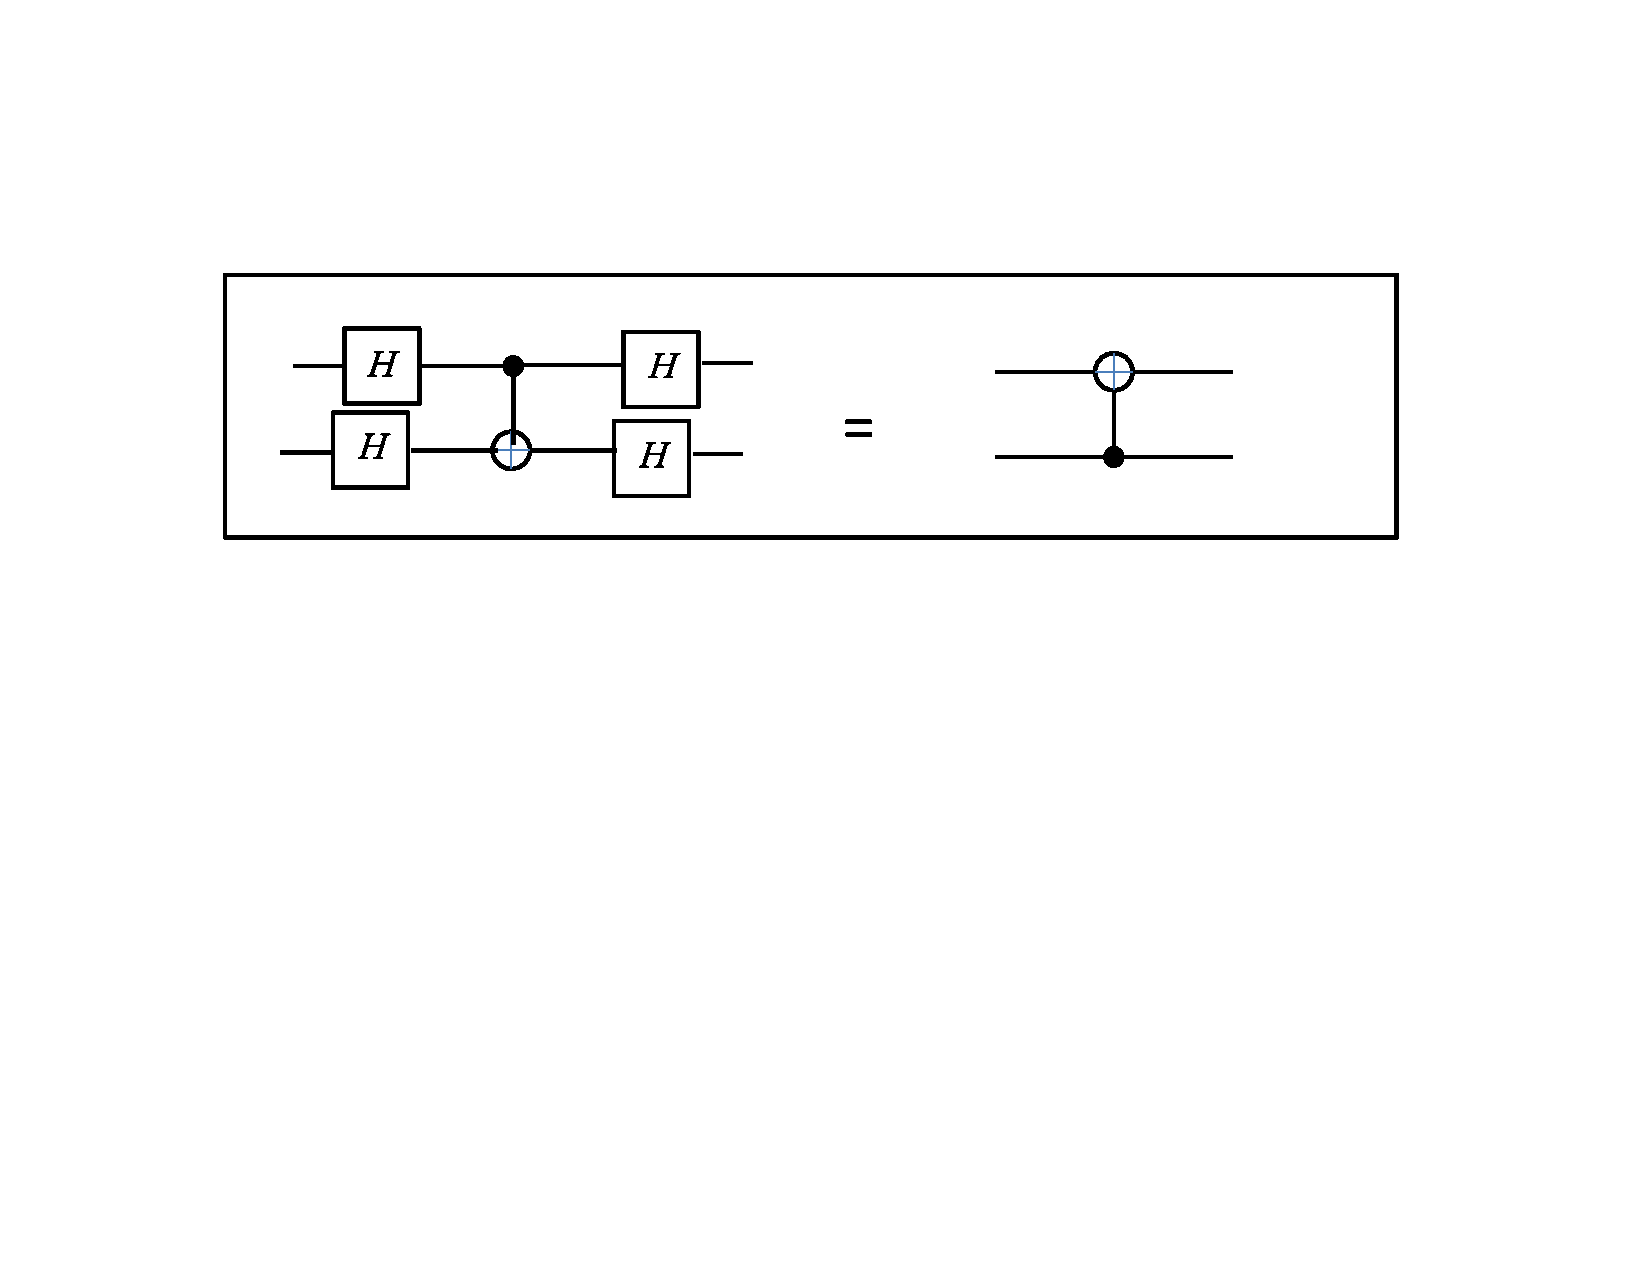
\includegraphics[width=400pt]{fig1-4-1.pdf}
    \end{center}
\end{problem}

\begin{solution}
    \vfill
\end{solution}

\end{document}

